\label{Julian}
\subsection{Creator}
Der 'Creator' wurde dazu entwickelt, um dem Benutzer die Möglichkeit zu geben, einen Self-Assesment-Test zu erstellen ohne die dafür anderweitig nötigen Kenntnisse in XML zu besitzen bzw. es ihm zu erleichtern, auch wenn er sie besitzt. Das Programm verfügt über weitreichende Funktionen, damit der Test die benötigten Eigenschaften bieten kann. In diesem Abschnitt werden diese Funktionen erläutert und eine Gesamtübersicht über das Programm gegeben. 

\subsubsection*{Übersicht}
%hier übersichtsbild einfügen
\begin{figure}[htbp] 
  \centering
     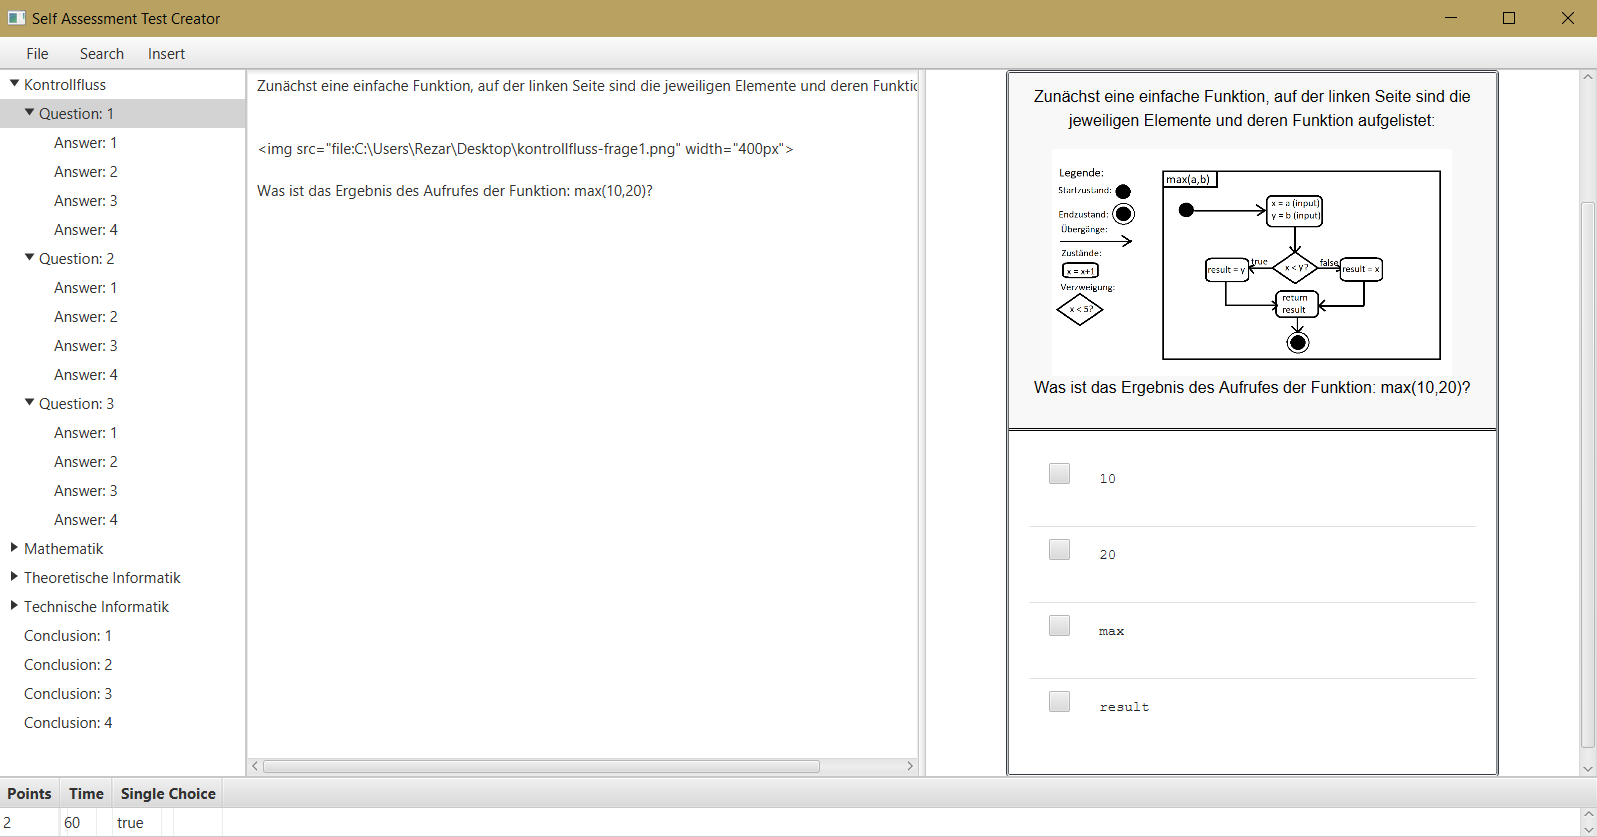
\includegraphics[width=0.5\textwidth]{Julian_Images/Creator-Uebersicht.png}
  \caption{}
  \label{fig:Bild0}
\end{figure}
Das Haupt-Fenster des Creators beinhaltet fünf wichtige Elemente die zur Übersicht und Erstellung des Testes dienen. Auf der linken Seite ist ein 'TreeView', der die Struktur des Testes darstellt. In ihm werden die Kategorien, deren zugehörigen Fragen, Antworten und die Folgerungen angezeigt. Jedes 'TreeItem', das in ihm existiert, repräsentiert ein Java-Objekt der zugehörigen Klasse, dessen Name in den 'TreeItems' angezeigt wird.
\\
\\
In der Mitte gibt es ein großes Textfeld, das das Inhaltsattribut des zugehörig ausgewählten 'TreeItems' wiedergibt. In ihm kann man dieses mithilfe von HTML und Markdown editieren bzw. nach belieben verändern.
\\
\\
Im unteren Bereich wird eine Tabelle erstellt, die alle Attribute des im 'TreeView'  ausgewählten Elements anzeigt. Diese Attribute variieren je nach dem welche Klasse das Element besitzt. Kategorien besitzen als Attribut ihren Namen, Fragen hingegen haben die Attribute Punkte und Zeit, Folgerungen enthalten das Attribut Umfang.
\\
\\
Die obere Leiste enthält 'MenuItems' mit mehreren Funktionen, die in einem späteren Abschnitt näher betrachtet werden.
\\
\\
Auf der rechten Seite gibt es ein großes Feld, dessen Funktion darin besteht, aus den im 'TreeView' ausgewählten Fragen und deren Antworten ein HTML-Dokument zu erstellen und anzuzeigen, damit der Benutzer sehen kann, wie die Website am Ende aussehen wird. Dieses Feld wird immer aktualisiert, sobald der Benutzer in dem Textfeld etwas verändert oder ein anderes Element im 'TreeView' ausgewählt wird.
\\
\\
Der Balken zwischen dem Textfeld und der Seitengenerierung ist dazu, da die Größe jedes Feldes beliebig anzupassen, außerdem kann der Benutzer die Größe des gesamten Fensters ohne Probleme nach belieben verändern.

\subsubsection*{Funktionen}
Unter der Kategorie 'File' gibt es neun Buttons, die nach Funktionen sortiert und mit 'SeparatorItems' voneinander getrennt sind. Die ersten vier, also 'New Category', 'New Question', 'New Answer' und 'New Conclusion', erstellen die jeweils zugehörigen 'TreeItems', die anschließend im 'TreeView' angezeigt werden. 'Delete Item' entfernt ein ausgewähltes 'TreeItem' und dessen zugehöriges Java Objekt. Die bisher aufgezählten Funktionen sind auch in einem 'ContextMenu' des 'TreeViews' zu finden. 'Generate Website' erstellt einen Zip-Ordner, der HTML, Javascript und CSS-Dateien enthält, die später zur Erstellung der Webseite des Servers dienen. Die zwei 'MenuItems' 'Import XML' und 'Export XML' fragen den Benutzer nach einer XML-Datei, in die der Inhalt gelesen bzw. gespeichert wird. Das letzte 'MenuItem' 'Exit'  beendet das Programm, dabei wird der Benutzer zu einer Bestätigung aufgefordert.
\\
\\
Die zweite Kategorie 'Search' enthält zwei Funktionen, die jeweils neue Fenster aufrufen, mit denen der Benutzer in dem großen Textfeld nach einem beliebigen Text suchen bzw. ihn ersetzen kann. Dabei kann er auch die Option auswählen, Groß- und Kleinschreibung nicht zu beachten. 
\\
\\
Die dritte und letzte Kategorie 'Insert' ist dazu da, Medien, also Bilder und/oder Videos, in das Textfeld einzufügen. Dabei wird der Benutzer danach gefragt eine Datei auszuwählen, deren Dateipfad anschließend in das Textfeld, an der Stelle, an dem sich der Cursor des Benutzers befindet, eingefügt wird. 
\\
\\
